
\noindent\begin{minipage}{\textwidth}
    \begin{table}[H]
        \centering
        \caption{Hiperparâmetros e Resultados do Melhor Modelo - resnet\_v8\_AB\_opt\_aug}
        \vspace{0.2cm}
        \resizebox{\textwidth}{!}{%
            \begin{tabular}{ll | lrrr}
                \hline
                \multicolumn{2}{c|}{\textbf{Hiperparâmetros}} & \multicolumn{4}{c}{\textbf{Métricas por Classe}} \\ \hline
                \textbf{Parâmetro} & \textbf{Valor} & \textbf{Classe} & \textbf{Precisão} & \textbf{Recall} & \textbf{F1-Score} \\ \hline
    Agendador (Patience) & 3 & 31.2 & 0,1862 & 0,9912 & 0,3135 \\ 
Agendador de LR & ReduceLROnPlateau & 31.3 & 0,0870 & 0,0099 & 0,0178 \\ 
Architecture & resnet34 & 31.4 & 0,0000 & 0,0000 & 0,0000 \\ 
Augmentation (Método) & None & 32.3 & 0,3636 & 0,0204 & 0,0386 \\ 
Batch Size & 32 & 32.4 & 0,0000 & 0,0000 & 0,0000 \\ 
Decaimento de Peso (WD) & 0,0000 & 33.3 & 0,3333 & 0,0104 & 0,0201 \\ 
Dropout & 0,4353 & 41.4 & 0,0000 & 0,0000 & 0,0000 \\ 
Função de Perda & CrossEntropyLoss & 41.5 & 0,2222 & 0,0513 & 0,0833 \\ 
Hidden Units & 512 & 42.4 & 0,0000 & 0,0000 & 0,0000 \\ 
Label Smoothing & 0,1000 & 44.4 & 0,0000 & 0,0000 & 0,0000 \\ 
\cline{3-6} 
Otimizador & SGD & \textbf{Média (Macro)} & 0,2463 & 0,2162 & 0,1330 \\ 
Taxa de Aprendizado (LR) & 2,32e-03 & \textbf{MCC} & \multicolumn{3}{c}{0,1140} \\ 
Unfreeze Layers & 2 &  & & &  \\ 
            \hline
            \end{tabular}%
        }
    \end{table}

    \begin{figure}[H]
        \centering
        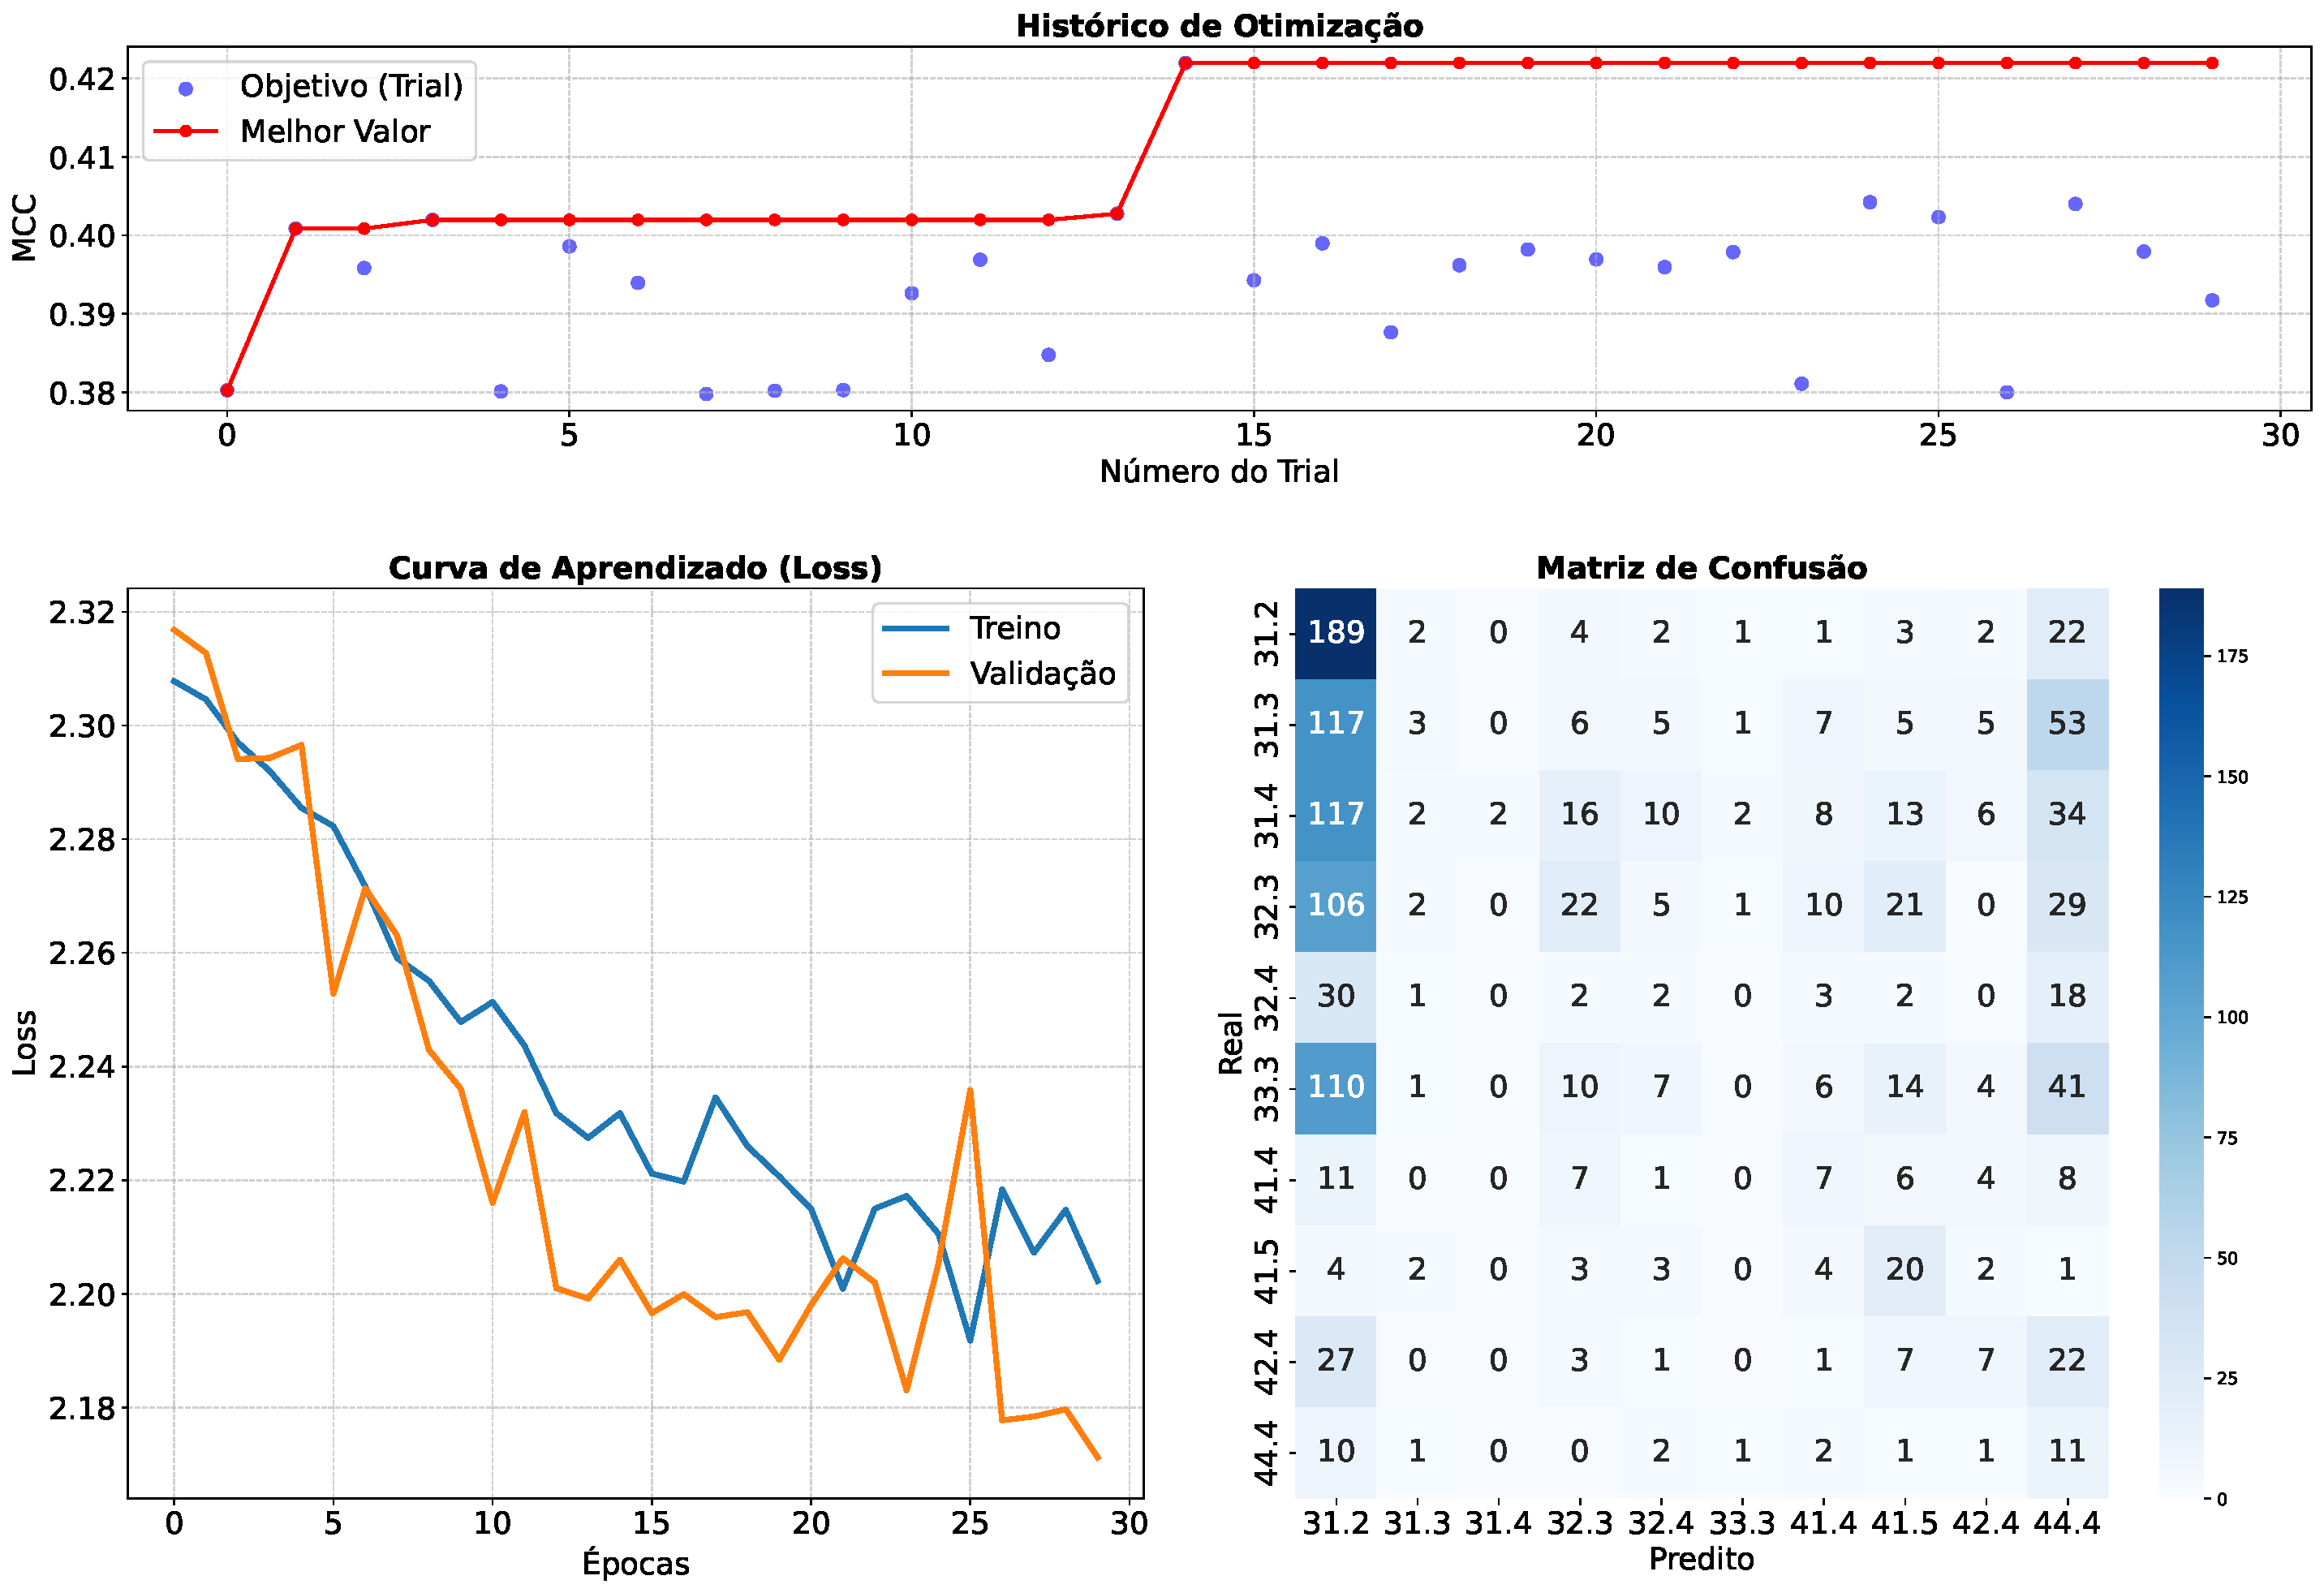
\includegraphics[width=0.85\textwidth]{tex/appendix/experiments/resnet_v8_AB_opt_aug/dashboard_consolidado.pdf}
        \caption{Histórico de Otimização, Curvas de Aprendizado e Matriz de Confusão - resnet\_v8\_AB\_opt\_aug}
    \end{figure}
\end{minipage}
\clearpage
